\section{Ajuste de distribuições e interpretação de dados de vento}\label{sec:vento}

\subsection{Apresentação breve da biblioteca e do ambiente}

Para a condução deste estudo de caso e a reprodução dos ajustes propostos, emprega-se a biblioteca \texttt{pyglam} (versão 1.1.0)~\cite{pyglam}, desenvolvida em Python e disponibilizada publicamente, e as distribuições clássicas da biblioteca \texttt{scipy.stats}~\cite{scipy2020}. O pacote implementa a parametrização FKML da família lambda generalizada e o seu ajuste pelo método dos momentos, descrito na seção~\ref{sec:gld}.

\rev{O fluxo de trabalho usa poucas funções da biblioteca:} \texttt{GlamFKML} usada para a instanciação do modelo paramétrico, \texttt{fit\_lambdas} para a execução do algoritmo de ajuste e os métodos \texttt{pdf} (função densidade de probabilidade), \texttt{cdf} (função distribuição acumulada) e \texttt{ppf} (função quantil, do inglês \textit{percent point function}). \rev{O método} \texttt{rvs} permite a geração de amostras aleatórias via transformação inversa. \rev{Um detalhe do desenho da biblioteca:} a função de ajuste retorna a solução do otimizador (\texttt{sol.x}), e o usuário instancia explicitamente o modelo ajustado (\texttt{modelo = GlamFKML(*sol.x)}), em vez de alterar a instância original.

\subsection{Origem, unidade e qualidade dos dados}

Os dados empíricos utilizados neste estudo são as velocidades médias diárias do vento (em m/s) da estação meteorológica automática A001 do Instituto Nacional de Meteorologia (INMET), em Brasília (DF), obtidas do Banco de Dados Meteorológicos do INMET~\cite{inmet2025}. A estação, de código OMM 86715, situa-se a cerca de $15{,}79^\circ$\,S e $47{,}93^\circ$\,W, a $1.161$\,m de altitude, e opera desde maio de 2000; foi a primeira estação automática da rede do INMET. O arquivo compreende o período de 06/05/2000 a 25/04/2025, com 9.121 registros diários sem datas repetidas; destes, 8.840 contêm a velocidade do vento e 281 estão vazios. Não há registros nulos ou negativos, e os valores \rev{aparecem no arquivo com passo de $0,1\,\text{m/s}$. Esse é o passo de registro (arredondamento) dos dados, que não deve ser confundido com a resolução metrológica do anemômetro, não documentada no arquivo.}

\rev{Os valores diários foram usados como fornecidos pelo BDMEP, no produto de dados diários de estações automáticas, em que o próprio INMET agrega os registros horários; os autores não recalcularam as médias. \textbf{[AUTORES: confirmar o nome exato do produto/consulta, a data do download, o critério de completude diária adotado pelo INMET e o fuso horário (UTC) dos registros horários.]} O vento é medido no mastro da estação, a 10\,m de altura \textbf{[AUTORES: confirmar na ficha da estação]}. Não foram encontradas no arquivo informações sobre troca de sensores ao longo do período, e essa possível fonte de heterogeneidade não pôde ser avaliada. As falhas não são isoladas: entre registros válidos de vento há 101 interrupções, a maior com 29 dias. A média mensal do vento varia de cerca de $2,10$ a $2,75\,\text{m/s}$ ao longo do ano; como todo o período é analisado em conjunto, o alvo aqui é a distribuição histórica agregada das médias diárias, e não a de uma estação do ano. Um quadro com essas informações e o script de leitura acompanham o material suplementar.}

As velocidades diárias válidas variam entre o mínimo de $0,7\,\text{m/s}$ e o máximo de $5,5\,\text{m/s}$, com média amostral de $2,345\,\text{m/s}$ e desvio padrão de $0,711\,\text{m/s}$ (calculado com divisor $n$).

\subsection{Caracterização exploratória}

\rev{Antes de ajustar qualquer modelo, convém olhar os dados.} A velocidade média diária do vento apresenta assimetria positiva, limitando-se inferiormente pelo zero físico e estendendo-se em uma cauda direita que acomoda dias excepcionalmente ventosos.

A figura~\ref{fig:exploratoria} mostra a série temporal e o histograma, evidenciando a concentração da massa de probabilidade na faixa de $1,5$ a $3,0\,\text{m/s}$. A tabela~\ref{tab:descritiva} \rev{reúne} as estatísticas descritivas dos dois estudos de caso, incluindo os quantis de 5\%, 50\% e 95\%, que servirão de referência numérica para avaliar as curvas ajustadas.

\begin{figure}[htbp]
\centering
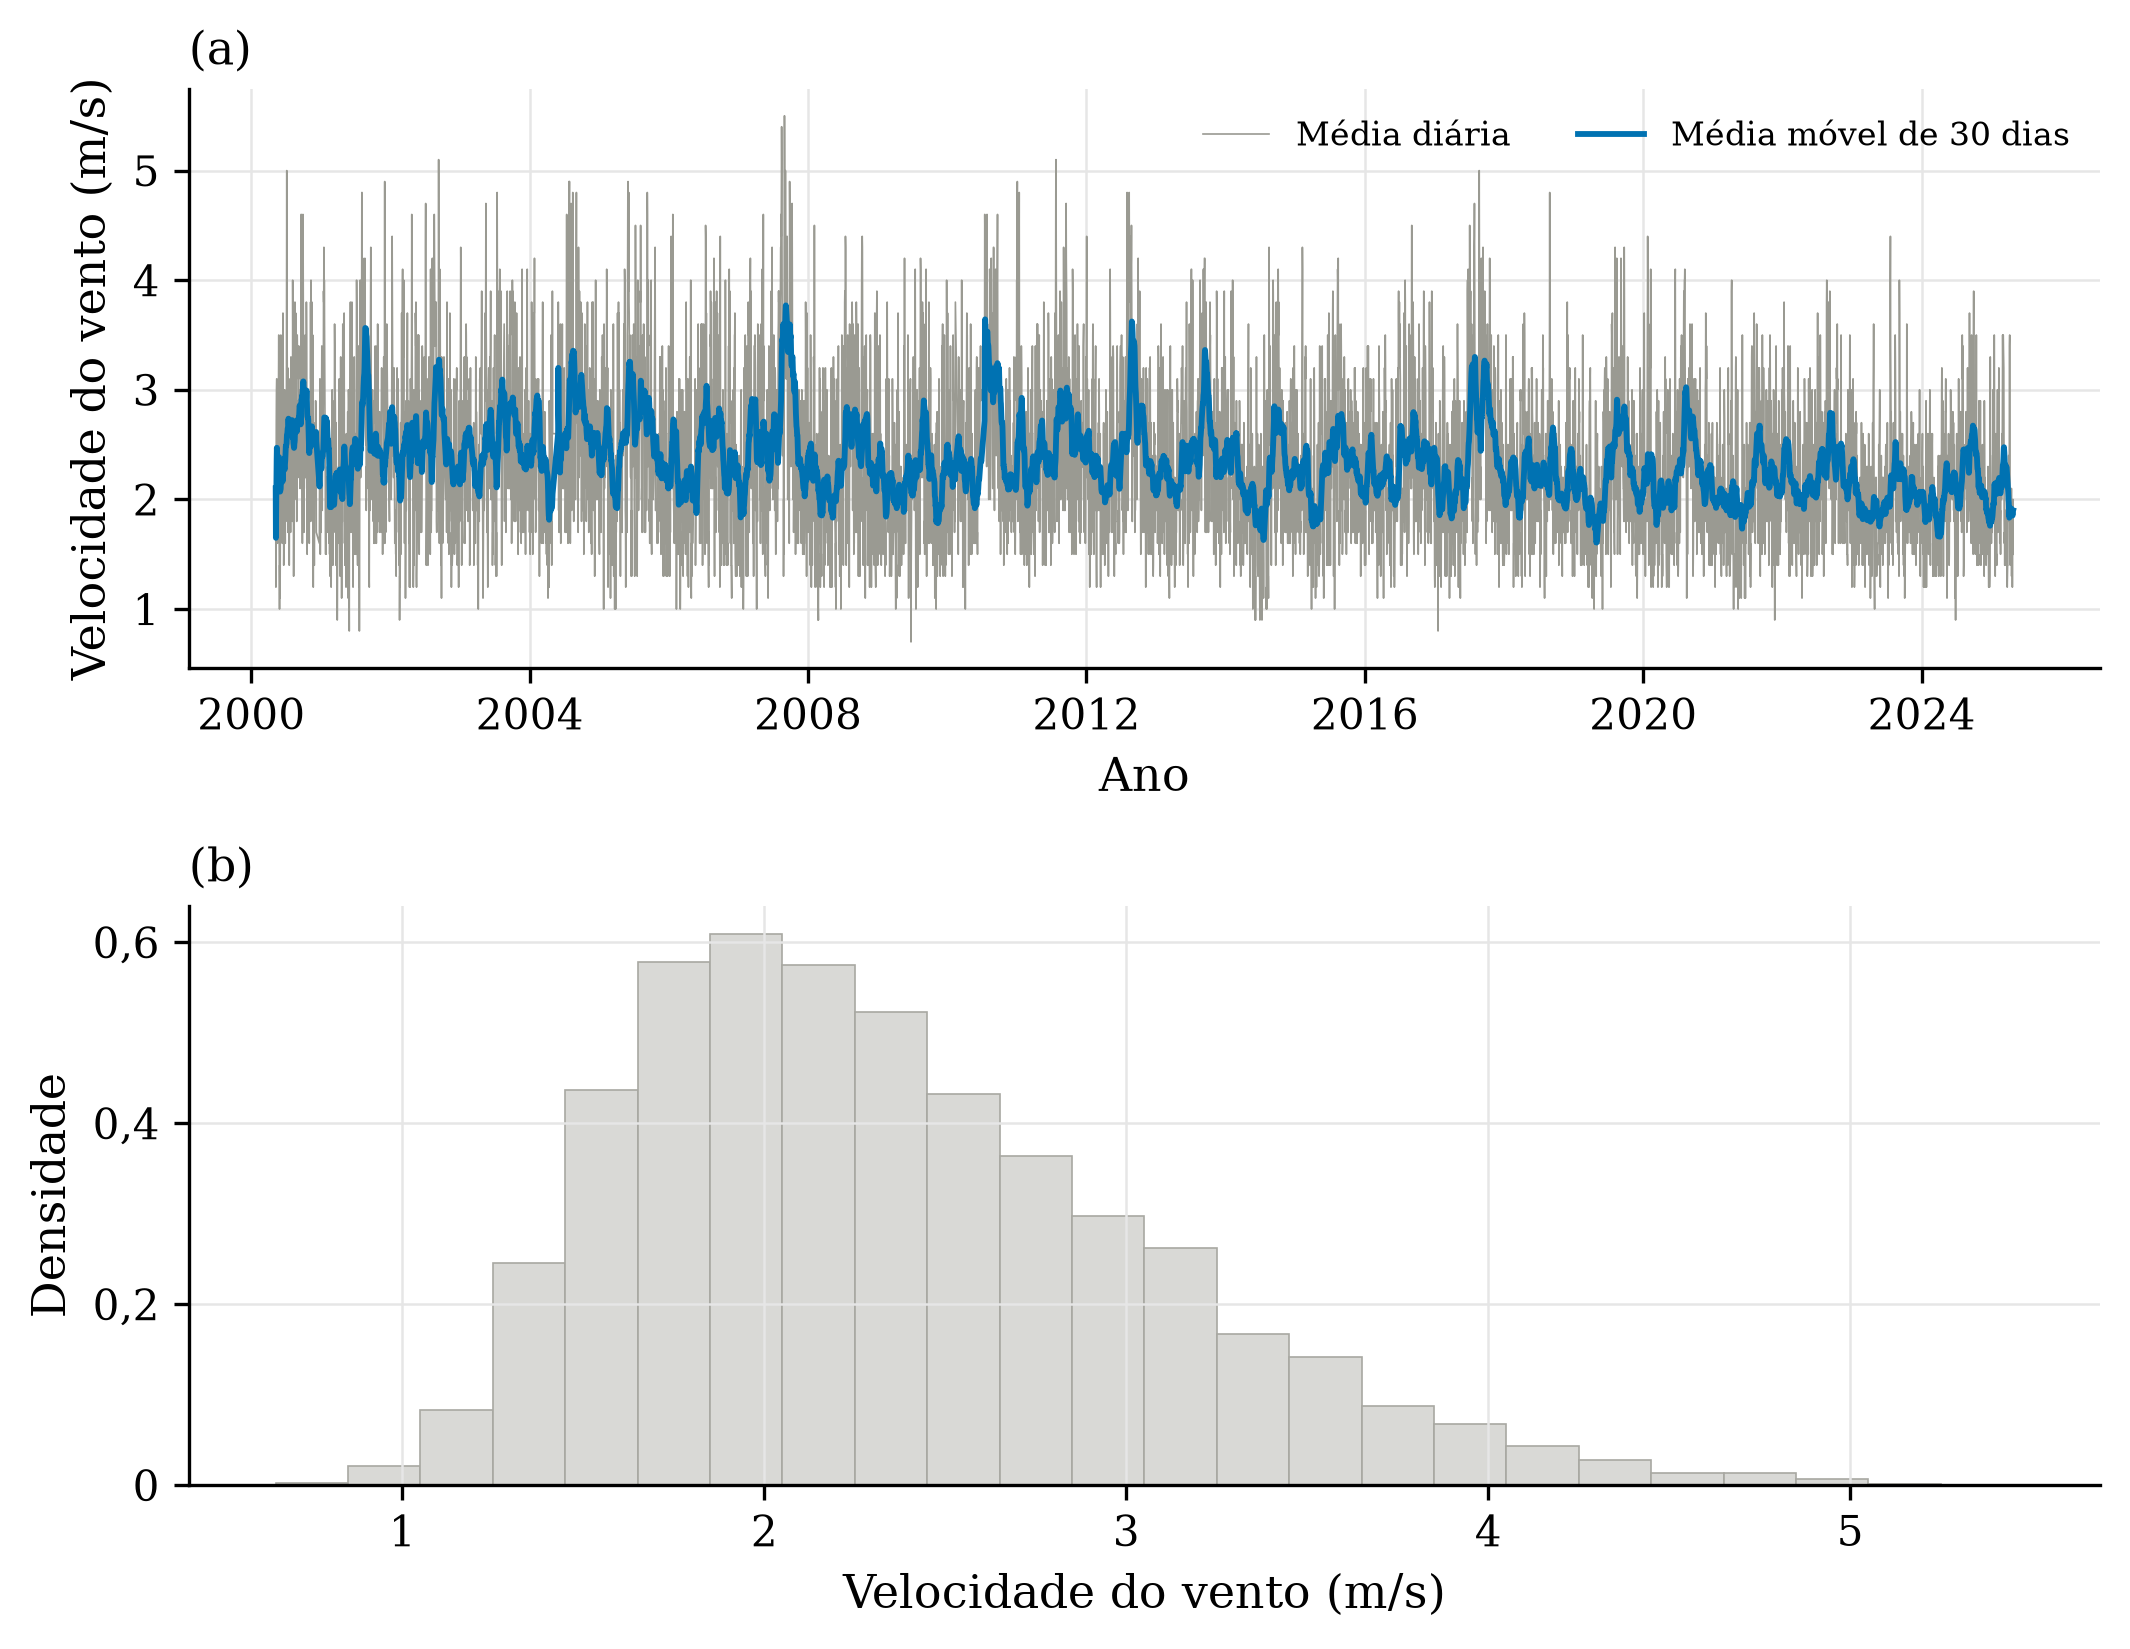
\includegraphics[width=0.85\textwidth]{figura2_vento_exploratoria_pt.png}
\caption{Velocidade média diária do vento na estação automática A001, em Brasília (DF), com (a) a série temporal e a média móvel de 30 dias e (b) o histograma.}
\label{fig:exploratoria}
\end{figure}

\begin{table}[htbp]
\centering
\caption{Estatísticas descritivas dos dois estudos de caso. Desvio padrão com divisor $n$ e curtose de Pearson (igual a $3$ para a normal). \rev{O coeficiente de variação não é dado para a temperatura: em graus Celsius a razão depende da origem arbitrária da escala (em kelvin, a mesma série daria cerca de $0,005$), e só tem leitura física para grandezas com zero físico, como a velocidade.}}
\label{tab:descritiva}
\small
\begin{tabular}{lcc}
\toprule
\textbf{Estatística} & \textbf{Vento (m/s)} & \textbf{Temperatura em julho ($^\circ$C)} \\
\midrule
$n$ & 8.840 & 768 \\
Média & 2{,}345 & 19{,}409 \\
Mediana & 2{,}20 & 19{,}50 \\
Desvio padrão & 0{,}711 & 1{,}466 \\
Coeficiente de variação & 0{,}303 & --- \\
Assimetria & 0{,}738 & -0{,}482 \\
Curtose (Pearson) & 3{,}368 & 3{,}717 \\
Mínimo; máximo & 0{,}7; 5{,}5 & 14{,}0; 23{,}2 \\
$Q_{0{,}05}$; $Q_{0{,}50}$; $Q_{0{,}95}$ & 1{,}40; 2{,}20; 3{,}70 & 16{,}84; 19{,}50; 21{,}70
\unskip \\
\bottomrule
\end{tabular}
\end{table}

\subsection{Famílias comparadas e estimação}

O ajuste estatístico compara três modelos paramétricos, a GLD-FKML (quatro parâmetros, estimada pelo método dos momentos) e dois modelos clássicos de referência com origem fixada no zero físico, a distribuição de Rayleigh (um parâmetro) e a distribuição de Weibull (dois parâmetros), ambas ajustadas por máxima verossimilhança.

A adoção da distribuição de Rayleigh no escopo atmosférico assume as hipóteses da seção~\ref{sec:dados} (componentes de vento gaussianas, ortogonais e independentes), formuladas para velocidades em intervalos curtos. Ao aplicá-la a médias diárias, testa-se deliberadamente um modelo fora do seu domínio de validade, o que é por si só uma lição sobre a importância da definição da variável. O estimador de máxima verossimilhança para esta família é $\widehat\sigma = \sqrt{\sum_{i=1}^n v_i^2 / (2n)}$, que fornece $\widehat\sigma = 1,733\,\text{m/s}$. No entanto, uma limitação estrutural surge imediatamente dos dados, pois o coeficiente de variação (CV) da distribuição de Rayleigh com origem em zero é uma constante, $\sqrt{(4-\pi)/\pi} \approx 0,523$, independentemente de $\sigma$. Em contrapartida, o CV empírico da amostra diária analisada é de $0,303$. Esta discrepância impede que o modelo de Rayleigh se adapte à forma da distribuição dos dados observados, qualquer que seja sua escala. Parte dela é esperada, porque a média de um dia combina dezenas de leituras e, por isso, varia relativamente menos de um dia para outro do que a velocidade em uma hora.

A introdução do modelo de Weibull flexibiliza essa restrição ao incorporar um parâmetro de forma (sendo a Rayleigh seu caso particular quando esse parâmetro vale $2$). O ajuste fornece forma $\widehat k = 3,448$ e escala $\widehat c = 2,605\,\text{m/s}$, o que oferece uma base de comparação mais justa com a flexibilidade dos quatro parâmetros da GLD-FKML.

Para a GLD-FKML, o sistema de equações não lineares do ajuste por momentos é sensível à aproximação inicial. O algoritmo explora por isso $15$ pontos de partida e aplica o critério de seleção descrito na seção~\ref{sec:gld}. Onze dos quinze pontos de partida convergiram para a mesma solução; \rev{duas tentativas terminaram em soluções válidas distintas entre si, ambas de resíduo maior,} e dois fora do domínio dos momentos. A solução selecionada, $\widehat{\boldsymbol\lambda} = (2,191;\, 1,727;\, \rev{0,555};\, 0,099)$, reproduz os quatro momentos da amostra. Como $\lambda_3$ e $\lambda_4$ são positivos, a equação~\eqref{eq:suporte} indica que o modelo ajustado tem suporte limitado, de $1,148$ a $8,057\,\text{m/s}$; a consequência desse resultado é discutida na seção~\ref{subsec:vento_interpretacao}.

O Código~\ref{lst:ajuste}, que continua o Código~\ref{lst:quantil}, executa esse ajuste, calcula os limites do suporte pela equação~\eqref{eq:suporte} e conta as observações que ficam fora dele.

\lstinputlisting[float=htbp, caption={Ajuste da GLD-FKML aos dados de vento pelo método dos momentos e verificação do suporte.}, label=lst:ajuste]{codigo/02_ajuste_momentos.py}

\subsection{O que medir e como ensinar a leitura do desempenho}

\rev{Sempre que possível, o desempenho deve ser lido na unidade da grandeza, e não só em números adimensionais. O diagnóstico usa duas medidas.}

\begin{enumerate}
    \item \textbf{Aderência global:} distância de Kolmogorov-Smirnov, $D_n = \sup_v |F_n(v) - \widehat{F}(v)|$, que quantifica o maior desvio absoluto entre a acumulada empírica e a do modelo.
    \item \textbf{Desvios nas caudas e no centro:} diferenças quantílicas $\Delta_p$ da equação~\eqref{eq:delta}, nos percentis $p \in \{0,05;\, 0,50;\, 0,95\}$. O sinal de $\Delta_p$ indica imediatamente se o modelo subestima (negativo) ou superestima (positivo) o vento, em m/s.
\end{enumerate}

O Código~\ref{lst:avaliacao} calcula as duas métricas para a GLD ajustada no Código~\ref{lst:ajuste}. Para os modelos de Rayleigh e de Weibull, basta trocar \texttt{gld} pela distribuição correspondente da biblioteca \texttt{scipy.stats}, que oferece os mesmos métodos \texttt{ppf} e \texttt{cdf}.

\lstinputlisting[float=htbp, caption={Desvios quantílicos e distância de Kolmogorov-Smirnov do modelo ajustado.}, label=lst:avaliacao]{codigo/03_avaliacao.py}

A tabela~\ref{tab:desempenho_vento} compila estas métricas. A figura~\ref{fig:diagnosticos} reúne a densidade, a função acumulada e o gráfico Q-Q, permitindo localizar em quais quantis cada modelo se afasta dos dados.

\begin{table}[htbp]
\centering
\caption{Desempenho dos modelos ajustados aos dados diários de vento. As diferenças de quantis $\Delta_p$ estão em m/s.}
\label{tab:desempenho_vento}
\begin{tabular}{lccccc}
\toprule
\textbf{Modelo} & \textbf{Parâmetros} & \textbf{$D_n$} & \textbf{$\Delta_{0,05}$} & \textbf{$\Delta_{0,50}$} & \textbf{$\Delta_{0,95}$} \\
\midrule
Rayleigh & 1 & 0{,}242 & -0{,}845 & -0{,}159 & +0{,}542 \\
Weibull & 2 & 0{,}085 & -0{,}299 & +0{,}142 & -0{,}119 \\
GLD-FKML & 4 & 0{,}041 & -0{,}025 & +0{,}046 & -0{,}037
\unskip \\
\bottomrule
\end{tabular}
\end{table}

\begin{figure}[htbp]
\centering
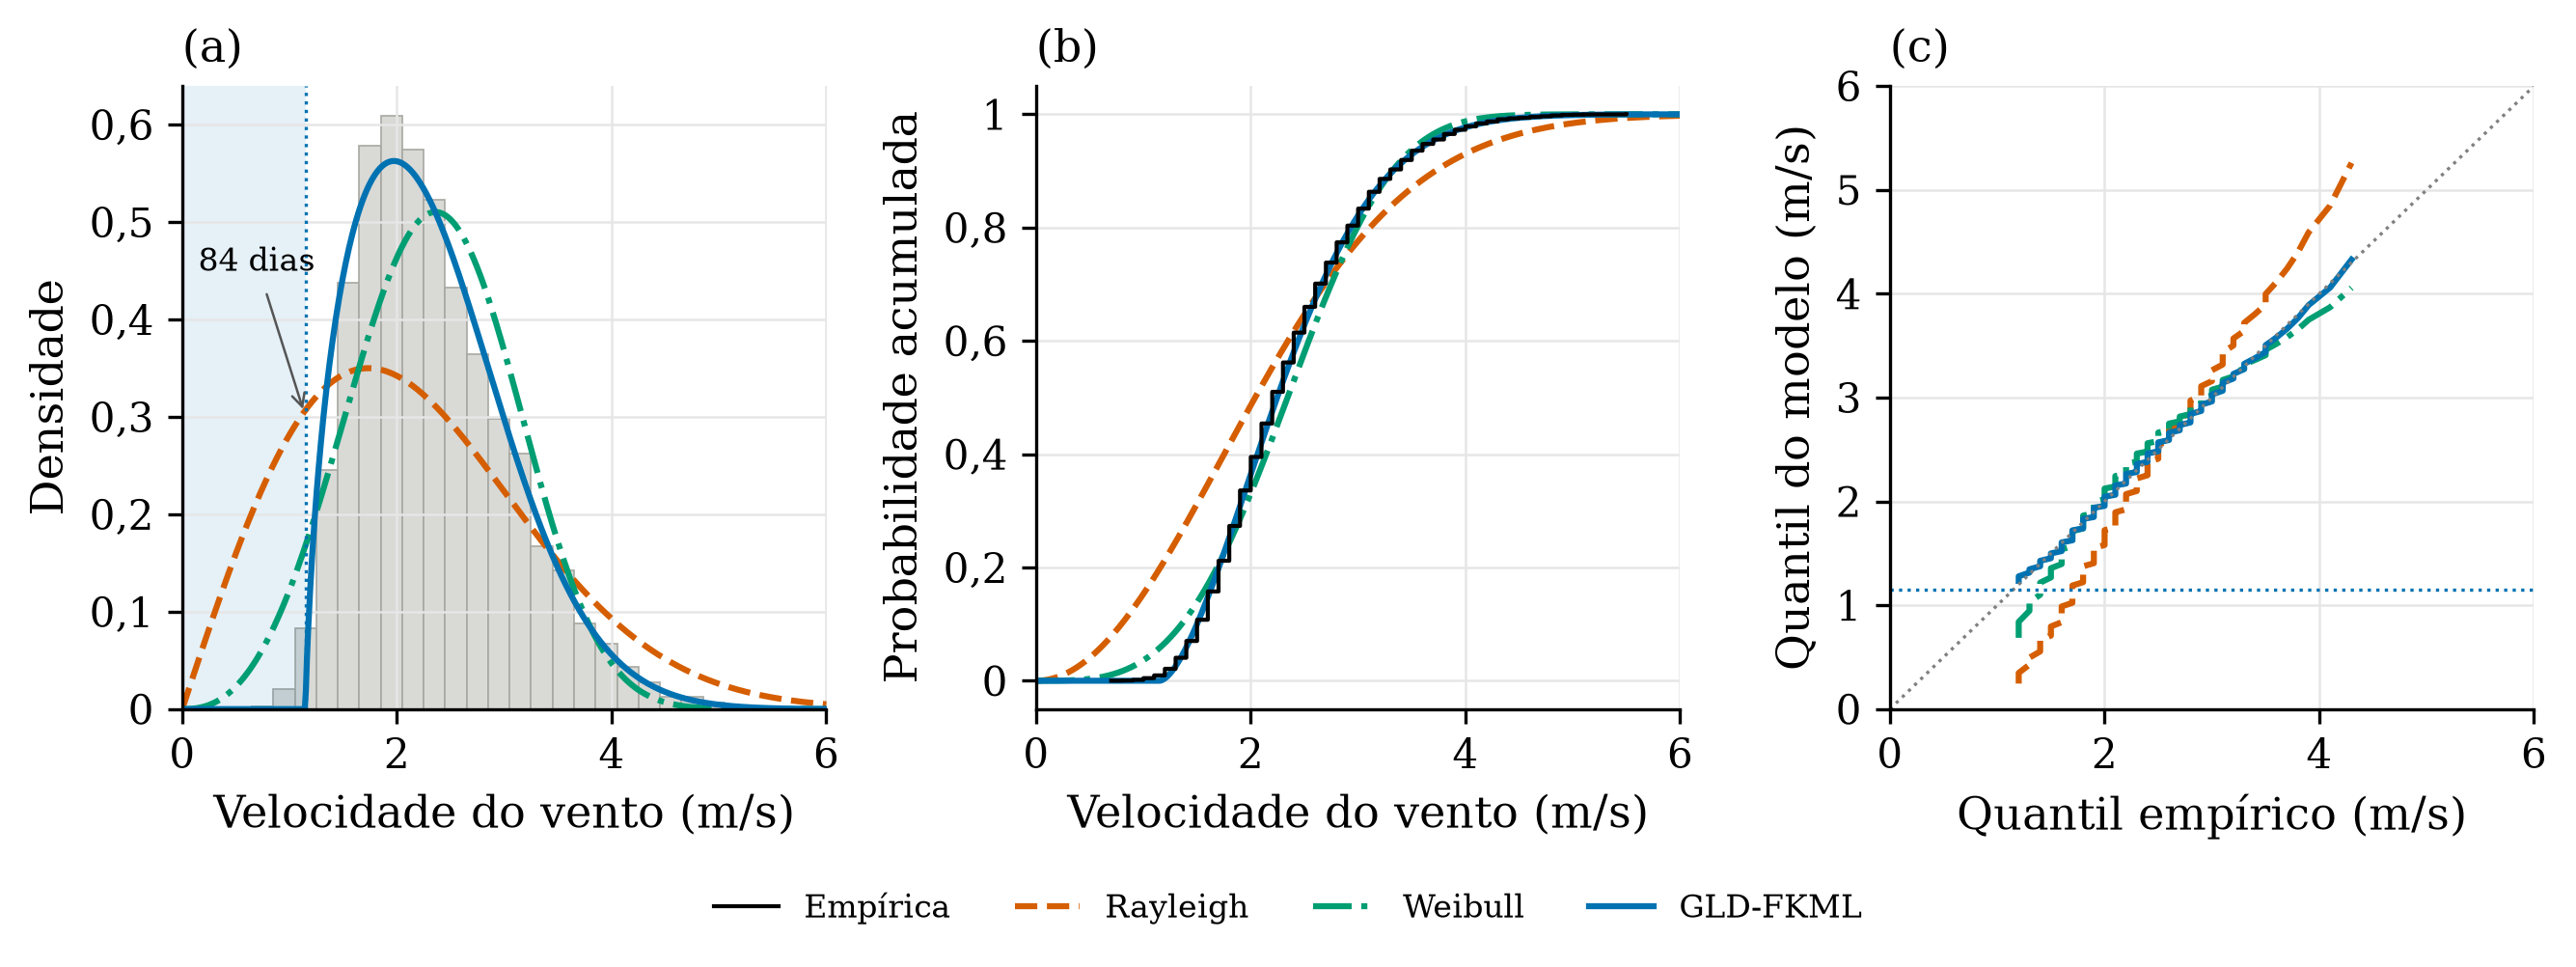
\includegraphics[width=\textwidth]{figura3_vento_diagnosticos_pt.png}
\caption{Diagnóstico comparativo dos modelos ajustados ao vento, com (a) densidades sobrepostas ao histograma, (b) funções distribuição acumuladas e (c) gráfico quantil-quantil, em que a linha pontilhada \rev{diagonal} indica concordância perfeita. \rev{A faixa sombreada em (a) e a linha horizontal em (c) marcam o limite inferior do suporte da GLD ($1,148\,\text{m/s}$); os 84 dias abaixo dele recebem probabilidade nula. O gráfico Q-Q usa os percentis de 1\% a 99\% e, por isso, não mostra esses dias.}}
\label{fig:diagnosticos}
\end{figure}

\subsection{Interpretação física e didática}\label{subsec:vento_interpretacao}

A leitura dos resultados revela que o coeficiente de variação fixo da distribuição de Rayleigh a torna larga demais para estes dados. Ela subestima o quantil de 5\% em $0,845\,\text{m/s}$ e a mediana em $0,159\,\text{m/s}$, e superestima o quantil de 95\% em $0,542\,\text{m/s}$, sendo inadequada para descrever o regime diário neste sítio. O modelo de Weibull melhora bastante a aderência, mas ainda erra o quantil de 5\% em $0,299\,\text{m/s}$ e a mediana em $0,142\,\text{m/s}$.

A GLD-FKML, que reproduz a assimetria e a curtose da amostra, reduz a distância $D_n$ à metade da obtida com a Weibull e mantém os três desvios quantílicos abaixo de $0{,}05\,\text{m/s}$, \rev{menores que o passo de registro} de $0{,}1\,\text{m/s}$ dos dados.

{\color{red}Para julgar se essas diferenças são relevantes, é preciso uma escala de comparação, e o arredondamento dos dados fornece a primeira. Como os registros têm passo de $0{,}1\,\text{m/s}$, a acumulada empírica avança em degraus, e nenhuma distribuição contínua consegue aproximá-la com $D_n$ arbitrariamente pequeno. Simulando amostras independentes de $8.840$ valores da própria GLD ajustada e arredondando-as a $0{,}1\,\text{m/s}$, obtém-se $D_n$ mediano de $0{,}034$, com $95\%$ das simulações abaixo de $0{,}039$, contra cerca de $0{,}008$ sem o arredondamento. No cenário simulado, portanto, o arredondamento sozinho leva $D_n$ a valores próximos do observado. Isso não decompõe o $D_n = 0{,}041$ da GLD em parcelas: o valor observado fica um pouco acima do percentil de 95\% da simulação, e a simulação ignora a dependência entre dias e o fato de os parâmetros terem sido estimados com os mesmos dados. A comparação dá a ordem de grandeza esperada, não um teste.

A segunda escala é a variabilidade amostral. A velocidade média de um dia está correlacionada com a do dia seguinte (autocorrelação de $0{,}65$ entre pares de dias consecutivos no calendário). Removido o ciclo anual, a autocorrelação cai abaixo de $0{,}1$ a partir de cerca de cinco dias, o que motivou blocos de dez dias no \textit{bootstrap}. Os blocos são sorteados apenas em trechos do calendário sem falhas, de modo que nenhum bloco junta datas separadas por uma lacuna; com blocos de 5, 20 ou 30 dias os resultados mudam pouco (desvio padrão de $0{,}021$ a $0{,}026\,\text{m/s}$ para a mediana e de $0{,}053$ a $0{,}060\,\text{m/s}$ para o quantil de 95\%). Em cada reamostra os dois modelos foram reajustados, de modo que a tabela~\ref{tab:incerteza_vento} mostra a variabilidade do próprio desvio $\Delta_p$, e não apenas a do quantil empírico.\par}

\begin{table}[htbp]
\color{red}
\centering
\caption{Desvios quantílicos $\Delta_p$ (m/s) da Weibull e da GLD-FKML e, entre parênteses, o desvio padrão de $\Delta_p$ em 500 reamostras \textit{bootstrap} em blocos de dez dias, com reajuste dos modelos em cada reamostra.}
\label{tab:incerteza_vento}
\begin{tabular}{lccc}
\toprule
\textbf{Modelo} & \textbf{$\Delta_{0,05}$} & \textbf{$\Delta_{0,50}$} & \textbf{$\Delta_{0,95}$} \\
\midrule
Weibull & -0{,}299 (0{,}011) & +0{,}142 (0{,}021) & -0{,}119 (0{,}038) \\
GLD-FKML & -0{,}025 (0{,}010) & +0{,}046 (0{,}020) & -0{,}037 (0{,}036)
\unskip \\
\bottomrule
\end{tabular}
\end{table}

{\color{red}Na mediana e no quantil de 95\%, os desvios da GLD ($+0{,}046$ e $-0{,}037\,\text{m/s}$) são da mesma ordem que os desvios padrão de reamostragem ($0{,}020$ e $0{,}036\,\text{m/s}$), enquanto o desvio da Weibull na mediana ($+0{,}142\,\text{m/s}$) é cerca de sete vezes maior que o seu. O quantil de 5\% pede mais cuidado. Por causa do arredondamento, o quantil empírico de 5\% vale $1{,}4\,\text{m/s}$ em todas as reamostras, e o seu desvio padrão bootstrap é nulo; isso diz respeito à grade dos registros, e não significa que o quantil da velocidade contínua seja conhecido sem incerteza. Os quantis dos modelos ajustados, que são contínuos, variam cerca de $0{,}01\,\text{m/s}$ entre reamostras. A diferença de $-0{,}299\,\text{m/s}$ da Weibull nesse quantil é grande diante de qualquer uma dessas escalas; a de $-0{,}025\,\text{m/s}$ da GLD é menor que o passo de registro. Essas comparações são descritivas: indicam uma diferença de forma da Weibull que não se explica pela variabilidade amostral, mas não constituem um teste de significância.\par}

\rev{Do ponto de vista didático, é preciso também examinar} o suporte do modelo ajustado. O limite inferior de $1{,}148\,\text{m/s}$ é positivo, o que evita atribuir probabilidade a velocidades negativas, mas está acima do menor valor observado, e $84$ dias da amostra ($0{,}95\%$) registraram velocidades menores, às quais o modelo atribui probabilidade nula. Uma consequência quantitativa é que a verossimilhança dos dados sob a GLD ajustada é nula, e o seu logaritmo, $-\infty$; critérios baseados na verossimilhança, como o de Akaike, não podem sequer ser calculados para comparar esse ajuste com o de Weibull. O ajuste por momentos reproduz os quatro resumos da amostra, mas nada no método obriga o suporte a conter todas as observações, ao contrário do que ocorre com a estimação por máxima verossimilhança. A lição central do exemplo é que a qualidade global do ajuste não dispensa a verificação da cauda relevante para a aplicação.

Por fim, os dados analisados são médias diárias. Eles descrevem a variabilidade de um dia para outro, mas não permitem recuperar a distribuição das velocidades em intervalos curtos, que é a relevante para estimar a densidade de potência eólica, proporcional a $\langle v^3 \rangle$. Com dados horários, a formulação por quantis oferece um caminho direto para esse cálculo, pois $\langle v^3 \rangle = \int_0^1 Q(u)^3\,du$, uma extensão natural do exemplo como exercício.
